\documentclass[10pt,twocolumn,letterpaper]{article}
\usepackage[margin=0.72in,columnsep=0.24in]{geometry}
\usepackage{mathptmx}
\usepackage[T1]{fontenc}
\usepackage{graphicx}
\usepackage{booktabs}
\usepackage{multirow}
\usepackage{amsmath}
\usepackage{xcolor}
\usepackage{caption}
\usepackage{enumitem}
\usepackage{titlesec}
\usepackage{fancyhdr}
\usepackage{tikz}
\usetikzlibrary{arrows.meta,positioning}
\usepackage[hidelinks]{hyperref}

\captionsetup{font=footnotesize,labelfont=sc,labelsep=period}
\captionsetup[table]{justification=centering,labelformat=simple,labelsep=newline,textfont=sc}
\renewcommand{\thetable}{\Roman{table}}
\titleformat{\section}{\centering\normalsize\scshape}{\Roman{section}.}{0.5em}{}
\titleformat{\subsection}{\normalsize\itshape}{\Alph{subsection}.}{0.5em}{}
\titlespacing*{\section}{0pt}{8pt}{4pt}
\titlespacing*{\subsection}{0pt}{6pt}{3pt}
\setlist{nosep,leftmargin=*}
\pagestyle{fancy}\fancyhf{}
\fancyhead[L]{\footnotesize [JOURNAL OR CONFERENCE NAME], 2026}
\fancyhead[R]{\footnotesize\thepage}
\renewcommand{\headrulewidth}{0pt}
\newcommand{\pholder}[1]{\textcolor{blue}{[#1]}}

\begin{document}

\twocolumn[
\begin{center}
{\LARGE Whole-Face Thermal Emotion Recognition on a Low-Cost,\\[2pt] Multi-Palette Dataset: Deep Models, Evaluation\\[2pt] Protocols and Session Confounds\par}
\vspace{8pt}
{\normalsize \pholder{Author 1}, \pholder{Author 2}, \pholder{Author 3}, and \pholder{Supervisor Name}\par}
\vspace{12pt}
\end{center}
]
{\renewcommand{\thefootnote}{}\footnotetext{The authors are with the Department of \pholder{Department}, Ajay Kumar Garg Engineering College (AKGEC), Ghaziabad, Uttar Pradesh, India (e-mail: \pholder{corresponding author e-mail}).}}

\noindent\textbf{\textit{Abstract}---Facial infrared thermography offers a contact-free view of autonomic responses that accompany emotion, and low-cost thermal cameras now make such data easy to collect. We train and evaluate deep networks for five-class emotion recognition (anger, happiness, neutral, sadness, surprise) on the facial-emotion subset of the public Comprehensive Facial Thermal Dataset (2485 images, UNI-T UTi165A camera, five false-colour palettes). Before training we remove on-screen overlays that the camera burns into every image, including the recording date and time. With image-level five-fold cross-validation, a fine-tuned ConvNeXt-Tiny reached 95.7\,$\pm$\,1.0\% accuracy (macro F1 0.957) and EfficientNet-B0 reached 88.6\,$\pm$\,1.1\% (chance 20\%). However, the time stamps in the file names show that the images come from five recording sessions and 44 short recording bursts, and that most sessions contain only one or two emotions. When whole recording bursts were held out, accuracy fell to 15.8\,$\pm$\,5.0\%, and when the models were trained on four sessions and tested on the only session that contains all five emotions, accuracy was 34.9\% (EfficientNet-B0) and 36.3\% (ConvNeXt-Tiny). Image-level results on this dataset therefore mostly measure recognition of the recording context rather than of emotion. We recommend that thermal emotion studies report session- or person-independent results alongside image-level ones, and we release our code.}

\vspace{4pt}
\noindent\textbf{\textit{Index Terms}---Infrared thermography, facial thermal imaging, emotion recognition, deep learning, ConvNeXt, evaluation protocol, data leakage, shortcut learning.}

\section{Introduction}

\textsc{Emotional} states are accompanied by changes in autonomic nervous system (ANS) activity, and part of this activity is visible as changes in skin blood flow. Because the face is richly and unevenly vascularised, these changes appear as local temperature variations that a long-wave infrared (LWIR) camera can record without contact, without visible light and without the voluntary control that people have over their facial muscles~\cite{ioannou2014}. Facial thermography has therefore been proposed as a complement to visible-spectrum expression analysis in affective computing~\cite{corneanu2016}. The psychophysiological literature reports that the response is region-specific: the nose tip cools markedly during fear and psychological stress~\cite{levine2001,engert2014}, the forehead often warms under cognitive and emotional load, and the periorbital, cheek and chin regions show patterns that depend on the emotion and the stimulus~\cite{ioannou2014,kosonogov2017}.

Thermal cameras have become affordable, and low-cost devices are increasingly used in research. These cameras typically save false-colour screenshots rather than radiometric temperature matrices: the colour assigned to a temperature depends on a user-selected palette, the colour range is re-scaled for every frame, and the camera's display overlays (spot temperature, date and time, colour bar) are saved with the image. Public datasets recorded with such cameras, like the Comprehensive Facial Thermal Dataset used here~\cite{dataset,abuhussein2024}, are attractive because they are openly licensed, but their structure needs care before accuracies can be interpreted.

This paper reports a whole-face deep-learning study on this dataset and asks a question that precedes any regional analysis: \emph{how much of the accuracy obtained on such data reflects emotion, and how much reflects the recording context?} Its contributions are:
\begin{enumerate}
\item an overlay-aware preprocessing step that removes the date, time, spot temperature and colour bar that the camera writes into every image;
\item fine-tuned ImageNet-pretrained networks (EfficientNet-B0 and ConvNeXt-Tiny) that reach 88.6\% and 95.7\% five-class accuracy under the image-level protocol common in the literature;
\item an analysis of the dataset's structure from the time stamps in the file names, which shows five recording sessions, 44 recording bursts and a strong confound between session and emotion label;
\item a comparison of three evaluation protocols showing that accuracy drops to chance level when whole recording bursts are held out and to 35--36\% on an unseen session;
\item released code that reproduces every number in the paper.
\end{enumerate}
Section~II reviews related work, Section~III describes the dataset, Section~IV the method and Section~V the results. Section~VI discusses the findings and limitations, and Section~VII concludes.

\section{Related Work}

\subsection{Physiological Basis and Regional Findings}
Facial skin temperature reflects local cutaneous perfusion under sympathetic control. Superficial vessels, such as those of the nose and of the supraorbital forehead, react faster and more visibly than deeper vessels~\cite{ioannou2014}. The nose tip is the most studied region: a sudden startle produces a temperature drop that is largest at the nose~\cite{levine2001}, and psychological stress produces a reliable ``nasal dip''~\cite{engert2014}, although findings for arousal are less consistent~\cite{kosonogov2017,salazar2015}. The forehead and nose often move in opposite directions under stress and load, and periorbital findings differ between studies~\cite{ioannou2014}. Recent reviews stress small samples, uncontrolled ambient conditions and inconsistent region definitions as the main obstacles to comparing studies~\cite{ioannou2014,nazzari2025}.

\subsection{Thermal Emotion Datasets}
The USTC-NVIE database~\cite{nvie} provides synchronised visible and thermal recordings of posed and spontaneous expressions of six basic emotions from more than 100 subjects. The KTFE database~\cite{ktfe} and its extension KTFEv2~\cite{ktfev2} contain spontaneous emotions elicited by audio-visual stimuli. Zhang et al.~\cite{zhang2016} recorded 140 subjects with a $640\times480$ LWIR camera during ten emotion-eliciting tasks. Kopaczka et al.~\cite{kopaczka2018,kopaczka2019} released 2935 high-resolution images of 90 subjects with landmarks and posed emotions. The I.Vi.T.E. database~\cite{esposito2022} contains film-induced expressions of 40 participants recorded at $160\times120$; its authors found that eye and nose temperatures did not reliably distinguish emotional states. Access to several of these datasets requires a signed agreement. The Comprehensive Facial Thermal Dataset~\cite{dataset,abuhussein2024} is openly licensed and was recorded with a low-cost camera in five palettes; to our knowledge no classification benchmark has been reported on its emotion subset.

\subsection{Thermal Facial Expression Recognition and Evaluation}
Approaches range from region temperatures with classical classifiers~\cite{cruz2017} to descriptors such as HOG~\cite{dalal2005} and deep convolutional networks~\cite{corneanu2016}. Kopaczka et al.\ reported 75.5\% accuracy for four posed emotions and 46.7\% for eight emotions with person-independent validation, against 42.0\% for human raters on the same images~\cite{kopaczka2019}. Across the literature, accuracy is substantially lower when test subjects are unseen. More generally, information shared between training and test sets other than the target, known as leakage, and models that exploit incidental cues instead of the intended signal, known as shortcut learning, are recognised causes of over-optimistic results in machine-learning-based science~\cite{kapoor2023,geirhos2020}.

\section{Dataset}

We use the facial-emotion subset of the Comprehensive Facial Thermal Dataset~\cite{dataset}, released under a CC~BY~4.0 licence and downloaded from Mendeley Data (version~1). Images were recorded with a UNI-T UTi165A camera (uncooled microbolometer, $160\times120$ pixels, 8--14\,\textmu m) and saved as $240\times320$-pixel BMP files (portrait) in five palettes: ironbow, rainbow, ice blue, red hot and white hot~\cite{abuhussein2024}. Expressions were at least partly posed~\cite{abuhussein2024}. Our copy contained 2485 labelled images; Table~\ref{tab:counts} gives the counts per emotion and palette. Two folder names in the archive are misspelt (``surpise'' and, for anger, ``IRNBOW''), and neutral images are stored as ``natural''; we mapped them to the intended labels.

\begin{table}[t]
\caption{Images per emotion and palette in the facial-emotion subset}
\label{tab:counts}
\centering\footnotesize
\setlength{\tabcolsep}{4pt}
\begin{tabular}{lrrrrrr}
\toprule
Emotion & Ironbow & Rainbow & Ice blue & Red hot & White hot & Total\\
\midrule
Anger     & 98  & 100 & 110 & 100 & 101 & 509\\
Happiness & 104 & 118 & 106 & 101 & 109 & 538\\
Neutral   & 92  & 119 & 105 & 110 & 115 & 541\\
Sadness   & 90  & 93  & 82  & 93  & 99  & 457\\
Surprise  & 90  & 91  & 82  & 86  & 91  & 440\\
\midrule
Total     & 474 & 521 & 485 & 490 & 515 & 2485\\
\bottomrule
\end{tabular}
\end{table}

\textbf{On-screen overlays.} Every image contains the camera's display overlay: the spot temperature and the recording date and time along the top edge, a battery icon, a crosshair at the centre and a colour bar with its maximum and minimum temperatures along the right edge (Fig.~\ref{fig:samples}, top). The date is a direct label leak whenever emotions were recorded on different days, and the colour-bar limits encode scene temperature.

\begin{figure}[t]
\centering
\IfFileExists{fig/samples.png}{\includegraphics[width=\columnwidth]{fig/samples.png}}{\fbox{\parbox[c][3cm][c]{0.9\columnwidth}{\centering\pholder{sample images}}}}
\caption{One image per palette as saved by the camera (top), including the spot temperature, date, time and colour bar, and the same images after the overlay crop used for training (bottom).}
\label{fig:samples}
\end{figure}

\textbf{Recording sessions and bursts.} The dataset contains no subject identifiers, but every file is named \texttt{imgYYYYMMDD\_HHMMSS}. The dates reveal five recording sessions, and Fig.~\ref{fig:sessions} shows that emotion and session are strongly confounded: on 2023-11-26 only happiness and neutral were recorded, on 2023-12-03 mostly anger, and on 2023-12-05 and 2023-12-10 only sadness and surprise. Only the session of 2024-03-03 (455 images) contains all five emotions in near-equal numbers. Grouping images of the same emotion whose time stamps lie less than 60\,s apart, across all palettes, gives 44 recording bursts (median 45 images, largest 180), each a continuous recording of one expression. The number of persons could not be established from the data.

\begin{figure}[t]
\centering
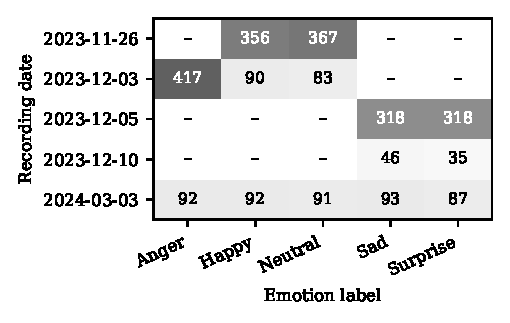
\includegraphics[width=\columnwidth]{fig/sessions.pdf}
\caption{Images per recording date (from the file names) and emotion label. Only the 2024-03-03 session contains all five emotions.}
\label{fig:sessions}
\end{figure}

\section{Method}

Fig.~\ref{fig:pipeline} summarises the pipeline.

\begin{figure}[t]
\centering
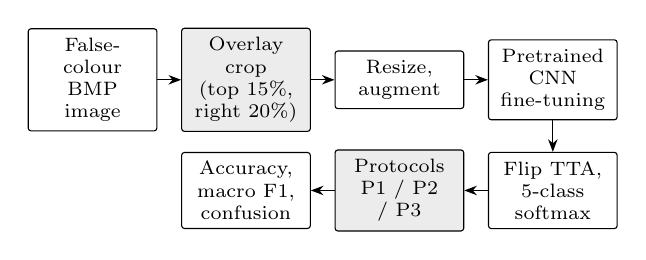
\begin{tikzpicture}[node distance=3mm, box/.style={draw, rounded corners=1pt, align=center, font=\scriptsize, minimum height=7mm, text width=14mm}, >={Stealth[length=1.6mm]}]
\node[box] (a) {False-colour\\BMP image};
\node[box, right=of a, fill=gray!15] (b) {Overlay crop\\(top 15\%,\\right 20\%)};
\node[box, right=of b] (c) {Resize,\\augment};
\node[box, right=of c] (d) {Pretrained\\CNN\\fine-tuning};
\node[box, below=4mm of d] (e) {Flip TTA,\\5-class\\softmax};
\node[box, left=of e, fill=gray!15] (f) {Protocols\\P1 / P2 / P3};
\node[box, left=of f] (g) {Accuracy,\\macro F1,\\confusion};
\draw[->] (a)--(b); \draw[->] (b)--(c); \draw[->] (c)--(d); \draw[->] (d)--(e); \draw[->] (e)--(f); \draw[->] (f)--(g);
\end{tikzpicture}
\caption{Overview of the method. Shaded steps are specific to this dataset: removing the camera's display overlays and choosing how images are split between training and test sets.}
\label{fig:pipeline}
\end{figure}

\subsection{Preprocessing}
Each image is converted to RGB and cropped by 15\% of its height at the top and 20\% of its width on the right, which removes the spot temperature, date and time, battery icon and colour bar while keeping the face (Fig.~\ref{fig:samples}, bottom). The centre crosshair is identical in every image and was left in place. Crops are resized to $256\times256$ pixels. All five palettes are used as they are, as three-channel images.

\subsection{Networks and Training}
Two ImageNet-pretrained~\cite{imagenet} networks from torchvision~\cite{pytorch} were fine-tuned end to end: EfficientNet-B0~\cite{efficientnet} (5.3\,M parameters) and ConvNeXt-Tiny~\cite{convnext} (28\,M parameters), each with a new five-way linear classifier. Training used AdamW~\cite{adamw} with weight decay $10^{-4}$, a learning rate of $10^{-4}$ for the pretrained layers and $10^{-3}$ for the new classifier, one epoch of linear warm-up followed by cosine decay, cross-entropy with label smoothing 0.1~\cite{szegedy2016}, batch size 32, mixed precision and at most 25 epochs. Training augmentation consisted of random resized crops to $224\times224$ (scale 0.75--1, aspect ratio 0.9--1.1), horizontal flips, rotations of up to $\pm10^\circ$, brightness and contrast jitter of $\pm15\%$ and random erasing ($p=0.25$, 2--12\% of the area)~\cite{zhong2020}. Hue and saturation were not changed, because colour encodes relative temperature. Within each training fold, about one seventh of the training groups (images under P1, recording bursts under P2 and P3; Section~IV-C) was held out as a validation set; the epoch with the highest validation macro F1 was kept, and training stopped after eight epochs without improvement. The test fold was never used for model selection. At test time, predictions for the image and its horizontal mirror were averaged. All experiments ran on a single NVIDIA T4 GPU in Google Colab; one ConvNeXt-Tiny fold took about 5.5\,min.

\subsection{Evaluation Protocols}
We compare three ways of assigning images to training and test sets:
\begin{itemize}
\item \textbf{P1, image level:} stratified five-fold cross-validation over images. We tried to keep near-duplicate frames together by perceptual hashing (256-bit difference hash, Hamming distance $\le 6$), but no image pair met that threshold, so P1 is equivalent to a random image-level split, as used in most work on datasets without subject identifiers.
\item \textbf{P2, burst level:} stratified grouped five-fold cross-validation in which all images of a recording burst (Section~III) stay in the same fold.
\item \textbf{P3, unseen session:} training on the four sessions recorded in 2023 (2030 images) and testing once on the 2024-03-03 session (455 images), which is the only session that contains all five emotions.
\end{itemize}
We report accuracy and macro-averaged F1 score; chance accuracy for five classes is 20\%. For P1 and P2 we give the mean and standard deviation over folds.

\section{Results}

\subsection{Image-Level Accuracy}
Table~\ref{tab:results} summarises all experiments. Under P1, ConvNeXt-Tiny reached 95.7\,$\pm$\,1.0\% accuracy (macro F1 0.957; folds 93.8, 96.8, 95.8, 96.2 and 96.0\%) and EfficientNet-B0 88.6\,$\pm$\,1.1\% (macro F1 0.885). Table~\ref{tab:perclass} and Fig.~\ref{fig:confusion} give the per-class results of ConvNeXt-Tiny. All classes exceeded 94\% recall; the most frequent confusions were sadness and surprise (12 images in each direction) and neutral images predicted as happiness (13 images). Accuracy also varied little between palettes: 98.1\% for ironbow, 97.7\% for white hot, 96.2\% for rainbow, 94.6\% for ice blue and 91.8\% for red hot.

\begin{table}[t]
\caption{Five-class accuracy and macro F1 under the three protocols (mean $\pm$ s.d.\ over folds for P1 and P2; chance 20\%)}
\label{tab:results}
\centering\footnotesize
\setlength{\tabcolsep}{4pt}
\begin{tabular}{llcc}
\toprule
Protocol & Network & Accuracy (\%) & Macro F1\\
\midrule
\multirow{2}{*}{P1 image level} & EfficientNet-B0 & 88.6 $\pm$ 1.1 & 0.885\\
 & ConvNeXt-Tiny & \textbf{95.7 $\pm$ 1.0} & \textbf{0.957}\\
\addlinespace
P2 burst level & EfficientNet-B0 & 15.8 $\pm$ 5.0 & 0.127\\
\addlinespace
\multirow{2}{*}{P3 unseen session} & EfficientNet-B0 & 34.9 & 0.323\\
 & ConvNeXt-Tiny & \textbf{36.3} & \textbf{0.339}\\
\bottomrule
\end{tabular}
\end{table}

\begin{table}[t]
\caption{Per-class results of ConvNeXt-Tiny under P1 (pooled over the five test folds, $n=2485$)}
\label{tab:perclass}
\centering\footnotesize
\begin{tabular}{lcccr}
\toprule
Emotion & Precision & Recall & F1 & Support\\
\midrule
Anger     & 0.986 & 0.941 & 0.963 & 509\\
Happiness & 0.963 & 0.972 & 0.968 & 538\\
Neutral   & 0.947 & 0.952 & 0.949 & 541\\
Sadness   & 0.938 & 0.958 & 0.948 & 457\\
Surprise  & 0.951 & 0.961 & 0.956 & 440\\
\midrule
Macro average & 0.957 & 0.957 & 0.957 & 2485\\
\bottomrule
\end{tabular}
\end{table}

\begin{figure}[t]
\centering
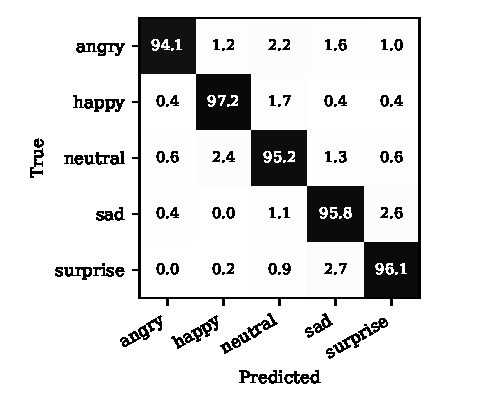
\includegraphics[width=0.86\columnwidth]{fig/confusion_p1_convnext.pdf}
\caption{Confusion matrix of ConvNeXt-Tiny under P1 (rows: true emotion; values in \% of the true class).}
\label{fig:confusion}
\end{figure}

\subsection{Burst- and Session-Independent Accuracy}
When whole recording bursts were held out (P2), EfficientNet-B0 fell to 15.8\,$\pm$\,5.0\% (folds 24.3, 17.1, 14.5, 14.0 and 9.1\%; macro F1 0.127), below chance level, and accuracy was below 19\% in every palette. During training, validation accuracy on held-out bursts also stayed near or below chance while training loss kept falling, which indicates memorisation of burst-specific appearance rather than learning of a transferable emotion cue. P2 was run with EfficientNet-B0 only.

When the networks were trained on the 2023 sessions and tested on the 2024-03-03 session (P3), accuracy was 34.9\% for EfficientNet-B0 (macro F1 0.323) and 36.3\% for ConvNeXt-Tiny (macro F1 0.339): clearly above the 20\% chance level, but far below the image-level results (Fig.~\ref{fig:protocols}). \pholder{Per-class recall under P3 is added from the saved prediction files.}

\begin{figure}[t]
\centering
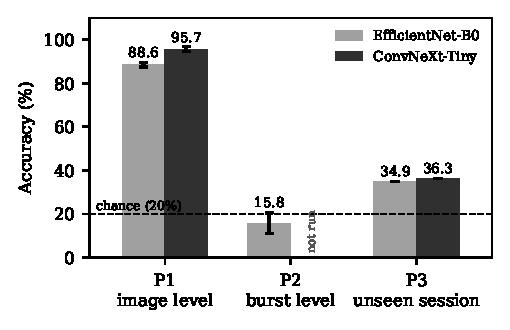
\includegraphics[width=\columnwidth]{fig/protocols.pdf}
\caption{Accuracy of the two networks under the three evaluation protocols. Error bars: s.d.\ over folds. The dashed line marks chance (20\%).}
\label{fig:protocols}
\end{figure}

\section{Discussion}

\subsection{What the Image-Level Accuracy Measures}
Under the image-level protocol, a modern pretrained network classifies this dataset almost perfectly. The other two protocols show that this figure says little about emotion recognition. Within a recording burst, consecutive frames show the same person, pose, clothing, background and colour scaling, so a random split places near-copies of most test images in the training set. Across bursts, the session--emotion confound (Fig.~\ref{fig:sessions}) allows a network to score highly by recognising the session: on the 2023-12-05 session, for example, only sadness and surprise occur. The result under P2, which is below chance, is consistent with this. A held-out burst is classified by its similarity to other bursts, and those come from sessions or persons whose labels are mostly different. This is the shortcut-learning pattern described by Geirhos et al.~\cite{geirhos2020}, and the overlay crop shows that even obvious shortcuts such as the printed date must be removed by hand.

P3 is the most meaningful of the three protocols for this dataset, because its test session contains all five emotions and was recorded months after the training data. The 35--36\% obtained there is a realistic estimate of what the networks learnt about emotion that transfers to a new recording session. ConvNeXt-Tiny was better than EfficientNet-B0 under both P1 and P3, but the gain under P3 (1.4 points on 455 images) is too small to be conclusive.

\subsection{Palettes}
The five palettes were pooled without conversion, and P1 accuracy was above 91\% in every palette, so the networks clearly cope with mixed palettes when the test images come from the same recording bursts. Whether palette normalisation improves generalisation across sessions is an open question for future work.

\subsection{Comparison With Previous Work}
Kopaczka et al.\ reported 75.5\% for four posed emotions and 46.7\% for eight emotions on high-resolution data with person-independent validation~\cite{kopaczka2019}, and Esposito et al.\ found that eye and nose temperatures did not reliably separate film-induced emotions~\cite{esposito2022}. Our P1 result of 95.7\% is far higher than these figures, but it is not comparable, because it is image-level. Our P3 result of 36.3\% for five classes is the closer comparison and lies below the person-independent results of Kopaczka et al., which were obtained with a much higher camera resolution.

\subsection{Recommendations}
For low-cost thermal emotion datasets we recommend: (i) inspect and crop on-screen overlays before training; (ii) recover the recording structure from file names or metadata and group images by burst, session or person when splitting; (iii) report at least one session- or person-independent result next to any image-level figure; and (iv) when collecting new data, record all emotions in every session and keep subject identifiers.

\subsection{Limitations}
(1) The dataset has no subject identifiers; bursts and sessions are proxies, and the number of persons is unknown. (2) Only one session contains all five emotions, so P3 rests on a single test session of 455 images and has no fold-to-fold variance estimate. (3) Expressions were posed, so part of what the networks detect may be the thermal footprint of muscle activity, such as an open mouth in surprise, rather than autonomic change. (4) Images are false-colour screenshots with per-frame scaling, so absolute temperatures are not available. (5) Only whole-face models were evaluated; P2 was run with EfficientNet-B0 only.

\subsection{Future Work}
The original aim of this project is a comparison of facial regions (forehead, periorbital, nose, cheeks, perioral and chin) across emotions. The results above show that such a comparison must be evaluated session-independently. The next steps are to invert the five palettes to a common relative-intensity scale, localise the six regions, test region-wise temperature changes with non-parametric statistics, train one classifier per region under P3, and compare where the network attends using Grad-CAM~\cite{gradcam}. Spontaneous emotions recorded with a radiometric camera and with subject identifiers would remove most of the limitations above.

\section{Conclusion}
We trained deep networks for five-class thermal emotion recognition on a public low-cost, multi-palette dataset. A fine-tuned ConvNeXt-Tiny reached 95.7\% accuracy under image-level cross-validation, but the same data analysed by recording session shows that this figure mainly reflects recognition of the recording context: accuracy was at chance when whole recording bursts were held out and 36.3\% on an unseen session containing all five emotions. Image-level results on datasets of this kind should therefore be reported together with session- or person-independent results, after on-screen overlays have been removed.

\section*{Data and Code Availability}
The Comprehensive Facial Thermal Dataset is available from Mendeley Data under a CC~BY~4.0 licence~\cite{dataset}. The training script (\texttt{thermal\_emotion\_train.py}) that produces every number in this paper is available at \url{https://github.com/anshul78-maker/thermal-emotion-recognition}.

\section*{Acknowledgment}
\pholder{Acknowledge your supervisor, department and the dataset authors.}

\footnotesize
\begin{thebibliography}{99}
\setlength{\itemsep}{0pt}
\bibitem{ioannou2014} S. Ioannou, V. Gallese, and A. Merla, ``Thermal infrared imaging in psychophysiology: Potentialities and limits,'' \emph{Psychophysiology}, vol.~51, no.~10, pp.~951--963, 2014.
\bibitem{corneanu2016} C. A. Corneanu, M. O. Simón, J. F. Cohn, and S. E. Guerrero, ``Survey on RGB, 3D, thermal, and multimodal approaches for facial expression recognition: History, trends, and affect-related applications,'' \emph{IEEE Trans. Pattern Anal. Mach. Intell.}, vol.~38, no.~8, pp.~1548--1568, 2016.
\bibitem{levine2001} J. A. Levine, I. Pavlidis, and M. Cooper, ``The face of fear,'' \emph{The Lancet}, vol.~357, no.~9270, p.~1757, 2001.
\bibitem{engert2014} V. Engert, A. Merla, J. A. Grant, D. Cardone, A. Tusche, and T. Singer, ``Exploring the use of thermal infrared imaging in human stress research,'' \emph{PLOS ONE}, vol.~9, no.~3, p.~e90782, 2014.
\bibitem{kosonogov2017} V. Kosonogov, L. De Zorzi, J. Honoré, E. S. Martínez-Velázquez, J.-L. Nandrino, J. M. Martinez-Selva, and H. Sequeira, ``Facial thermal variations: A new marker of emotional arousal,'' \emph{PLOS ONE}, vol.~12, no.~9, p.~e0183592, 2017.
\bibitem{salazar2015} E. Salazar-López \emph{et al.}, ``The mental and subjective skin: Emotion, empathy, feelings and thermography,'' \emph{Consciousness and Cognition}, vol.~34, pp.~149--162, 2015.
\bibitem{dataset} M. F. A. Abuhussein, A. Darwish, and A. E. Hassanien, ``Comprehensive facial thermal dataset,'' Mendeley Data, v1, 2024, doi:10.17632/8885sc9p4z.1.
\bibitem{abuhussein2024} M. F. A. Abuhussein, A. Darwish, and A. E. Hassanien, ``Exploring thermography technology: A comprehensive facial dataset for face detection, recognition, and emotion,'' arXiv:2407.09494, 2024.
\bibitem{nazzari2025} S. Nazzari, M. P. Pili, E. Çelik, S. Lucchin, and L. Provenzi, ``Infrared thermal imaging (ITI), a non-invasive window into early emotion regulation: A systematic review,'' \emph{Developmental Psychobiology}, 2025.
\bibitem{nvie} S. Wang \emph{et al.}, ``A natural visible and infrared facial expression database for expression recognition and emotion inference,'' \emph{IEEE Trans. Multimedia}, vol.~12, no.~7, pp.~682--691, 2010.
\bibitem{ktfe} H. Nguyen, K. Kotani, F. Chen, and B. Le, ``A thermal facial emotion database and its analysis,'' in \emph{Image and Video Technology (PSIVT 2013)}, LNCS vol.~8333. Springer, 2014, pp.~397--408.
\bibitem{ktfev2} H. Nguyen, N. Tran, H. D. Nguyen, L. Nguyen, and K. Kotani, ``KTFEv2: Multimodal facial emotion database and its analysis,'' \emph{IEEE Access}, vol.~11, pp.~17811--17822, 2023.
\bibitem{zhang2016} Z. Zhang \emph{et al.}, ``Multimodal spontaneous emotion corpus for human behavior analysis,'' in \emph{Proc. IEEE CVPR}, 2016, pp.~3438--3446.
\bibitem{kopaczka2018} M. Kopaczka, R. Kolk, and D. Merhof, ``A fully annotated thermal face database and its application for thermal facial expression recognition,'' in \emph{Proc. IEEE I2MTC}, 2018, pp.~1956--1961.
\bibitem{kopaczka2019} M. Kopaczka, R. Kolk, J. Schock, F. Burkhard, and D. Merhof, ``A thermal infrared face database with facial landmarks and emotion labels,'' \emph{IEEE Trans. Instrum. Meas.}, vol.~68, no.~5, pp.~1389--1401, 2019.
\bibitem{esposito2022} A. Esposito, V. Capuano, J. Mekyska, and M. Faundez-Zanuy, ``A naturalistic database of thermal emotional facial expressions and effects of induced emotions on memory,'' arXiv:2203.15443, 2022.
\bibitem{cruz2017} I. A. Cruz-Albarran, J. P. Benitez-Rangel, R. A. Osornio-Rios, and L. A. Morales-Hernandez, ``Human emotions detection based on a smart-thermal system of thermographic images,'' \emph{Infrared Physics \& Technology}, vol.~81, pp.~250--261, 2017.
\bibitem{dalal2005} N. Dalal and B. Triggs, ``Histograms of oriented gradients for human detection,'' in \emph{Proc. IEEE CVPR}, vol.~1, 2005, pp.~886--893.
\bibitem{kapoor2023} S. Kapoor and A. Narayanan, ``Leakage and the reproducibility crisis in machine-learning-based science,'' \emph{Patterns}, vol.~4, no.~9, p.~100804, 2023.
\bibitem{geirhos2020} R. Geirhos, J.-H. Jacobsen, C. Michaelis, R. Zemel, W. Brendel, M. Bethge, and F. A. Wichmann, ``Shortcut learning in deep neural networks,'' \emph{Nature Machine Intelligence}, vol.~2, pp.~665--673, 2020.
\bibitem{imagenet} J. Deng, W. Dong, R. Socher, L.-J. Li, K. Li, and L. Fei-Fei, ``ImageNet: A large-scale hierarchical image database,'' in \emph{Proc. IEEE CVPR}, 2009, pp.~248--255.
\bibitem{pytorch} A. Paszke \emph{et al.}, ``PyTorch: An imperative style, high-performance deep learning library,'' in \emph{Advances in Neural Information Processing Systems 32}, 2019.
\bibitem{efficientnet} M. Tan and Q. V. Le, ``EfficientNet: Rethinking model scaling for convolutional neural networks,'' in \emph{Proc. ICML}, 2019, pp.~6105--6114.
\bibitem{convnext} Z. Liu, H. Mao, C.-Y. Wu, C. Feichtenhofer, T. Darrell, and S. Xie, ``A ConvNet for the 2020s,'' in \emph{Proc. IEEE/CVF CVPR}, 2022, pp.~11976--11986.
\bibitem{adamw} I. Loshchilov and F. Hutter, ``Decoupled weight decay regularization,'' in \emph{Proc. ICLR}, 2019.
\bibitem{szegedy2016} C. Szegedy, V. Vanhoucke, S. Ioffe, J. Shlens, and Z. Wojna, ``Rethinking the Inception architecture for computer vision,'' in \emph{Proc. IEEE CVPR}, 2016, pp.~2818--2826.
\bibitem{zhong2020} Z. Zhong, L. Zheng, G. Kang, S. Li, and Y. Yang, ``Random erasing data augmentation,'' in \emph{Proc. AAAI}, 2020, pp.~13001--13008.
\bibitem{gradcam} R. R. Selvaraju, M. Cogswell, A. Das, R. Vedantam, D. Parikh, and D. Batra, ``Grad-CAM: Visual explanations from deep networks via gradient-based localization,'' in \emph{Proc. IEEE ICCV}, 2017, pp.~618--626.
\end{thebibliography}

\end{document}
